\section{Understanding Kiva website and Dataset}

\begin{itemize}
	\item Describe what user can do on the website: search for Projects, Auto-lending setup
	\item Describe how to get the data using GraphQL, Crawling method
	\item Describe data schema: fields that we can get, the meaning of each fields
	\item Describe preprocessing steps with the data
	      \begin{itemize}
		      \item Steps: accelerated loading, forming the big table, removing unwanted tags, remove anonymous Lenders, handle duplicates\dots
		      \item Forming the tri-partite graph: Lenders-Projects-Tags
		      \item Mention that we have to use CuDF for accelerated data handling
	      \end{itemize}
\end{itemize}

In this section, we will describe the Kiva website and the dataset that we use in this thesis.
We will also describe the preprocessing steps that we have to do with the dataset.

While there are many crowdfunding platforms,
we specifically choose Kiva because of its transparancy and the avalability of the data for public access.

\subsection{Kiva website}

To understand the data that the platform provides, we have to understand the interface that the platform provides to its users.
Like other platform, Kiva has a website where users can login and interact with the platform.
To understand the data that the platform provides and to extract meaningfull insight from the data,
we have to understand the interface that the platform provides to its users.

Any website interface is designed to make users interact with it in a pre-defined way.
In Kiva, we belived that the most function that users can do is to search for projects that they want to fund.
Or they can setup an Auto-Lending program, which will automatically fund projects that fit their criteria.


\begin{figure}[H]
	\centering
	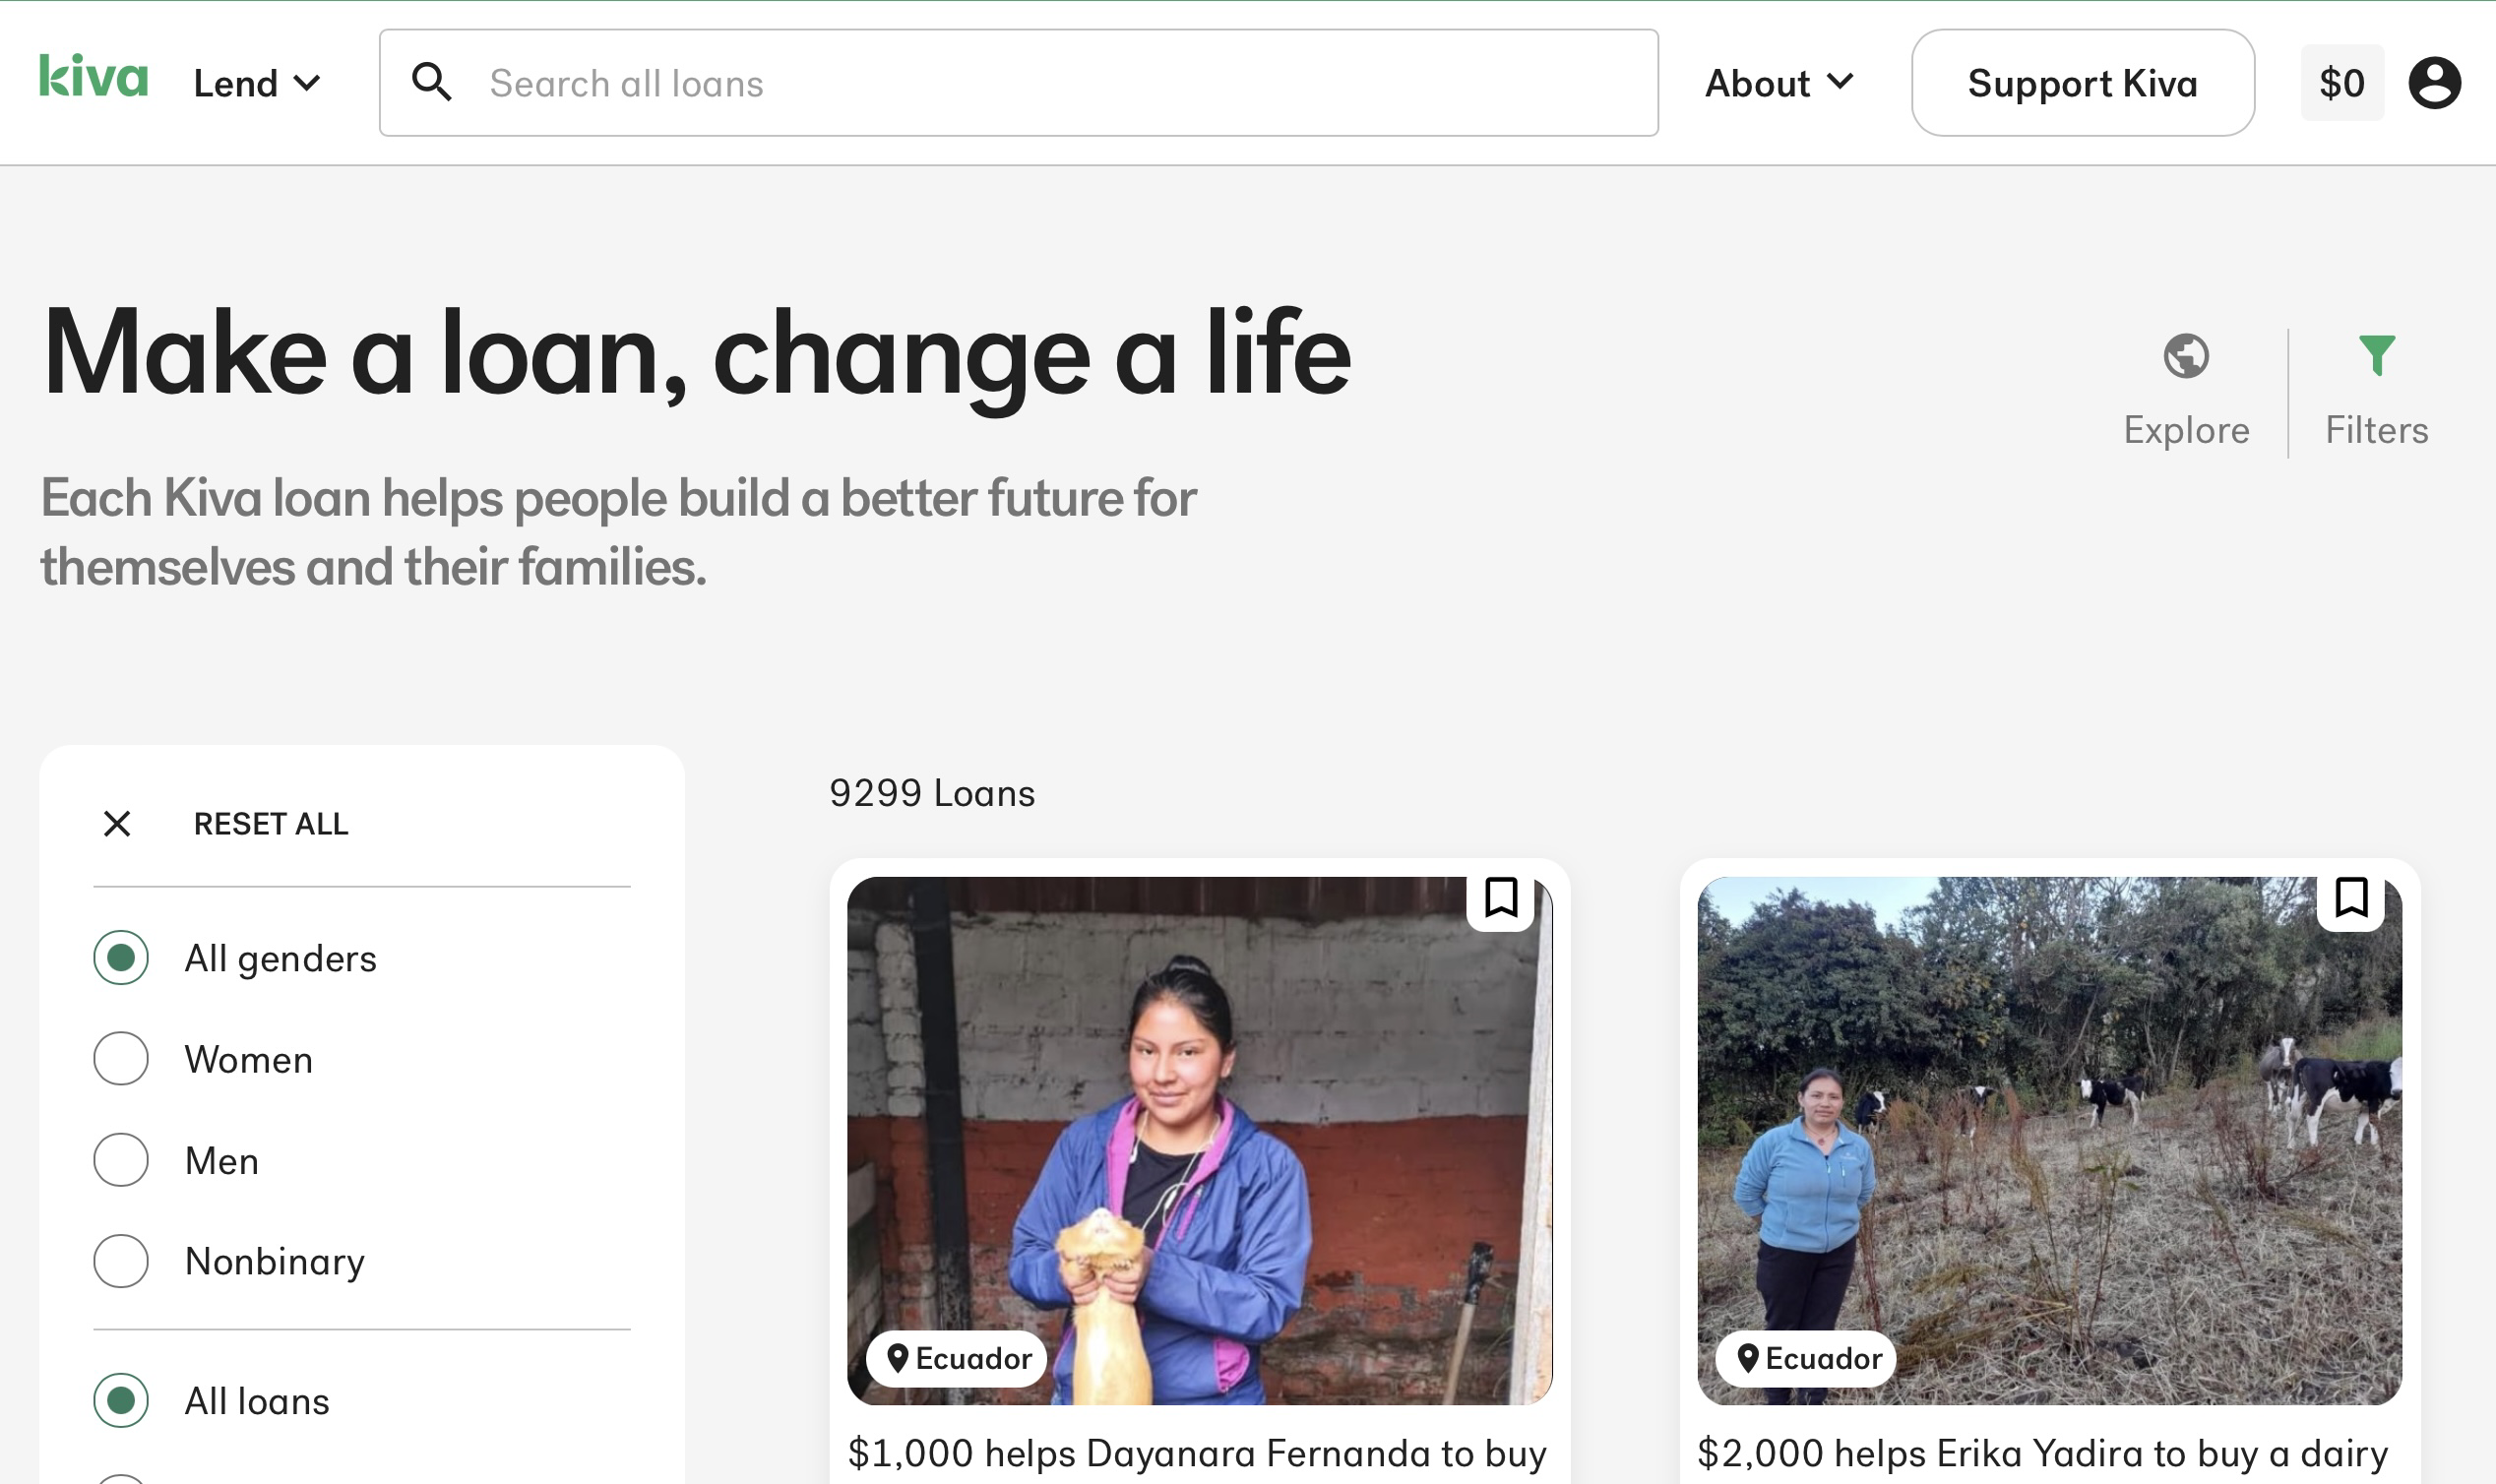
\includegraphics[width=0.8\textwidth]{images/kiva-browse-project.png}
	\caption{Kiva website interface for browsing projects}
	\label{fig:kiva-browser-project}
\end{figure}

It is important to know what Lenders can do when looking for his or her interested project.
Table \ref{tab:browser-criteria} shows the criteria that Lenders can use to filter the projects.
Later in the thesis, we will see that these criteria is not very align with the public data that the platform provide.
For example in the data, we could see some Tags that did not appear in the Tags list in the website.
We will consider these criteria as the gold standard for processing the data.

\begin{table}[H]
	\centering
	\resizebox{\textwidth}{!}{%
		\begin{tabular}{|c|c|c|c|}
			\hline
			   & Meaning                       & Type            & choices                                                                                                                 \\
			\hline
			1  & Gender of the borrower button & Choice          & Woman or Men or Nonbinary                                                                                               \\
			2  & Filter by type of Loan        & Choice          & Individual or Group                                                                                                     \\
			3  & Search by keyword             & Text            & Put any keyword to search in the stories of Projects                                                                    \\
			4  & Sort Order                    & Choice          & Amount: High to Low, Amount left, Amount: Low to High, Ending soon, Most recent, Trending now, Loan Length, Recommended \\
			5  & Location                      & Multiple choice & Choose from a list of countries                                                                                         \\
			6  & Sector                        & Multiple choice & Choose from a list of sectors                                                                                           \\
			7  & Attribute                     & Multiple choice & Choose from a list of attributes                                                                                        \\
			8  & Tags                          & Multiple choice & Choose from a list of tags                                                                                              \\
			9  & Loan Length                   & Choice          & All loans, 8 month or less, 16 months or less, 2 years or less, 2 years or more                                         \\
			10 & Loan Distribution             & Choice          & All loans, Parter, Direct                                                                                               \\
			11 & Partner Info                  & Text            & Search by Partner name                                                                                                  \\
			12 & Risk Rating                   & Range           & From 1 to 5                                                                                                             \\
			13 & Default Rate                  & Range           & From 0\% to 100\%                                                                                                       \\
			14 & Profitability                 & Range           & From -160\% to 90\%                                                                                                     \\
			\hline
		\end{tabular}%
	}
	\caption{Table with 4 columns \cite{kiva-browse}}
	\label{tab:browser-criteria}
\end{table}

Perhaps the most unique feature of Kiva is the Auto-Lending program.
In the program, Lenders can setup criterias for future projects that they want to fund.
When a new project is created, the platform will automatically fund the project if it fits the criterias.
Figure \ref{fig:auto-lend-setup} shows the interface for setting up the Auto-Lending program.

\begin{figure}[H]
	\centering
	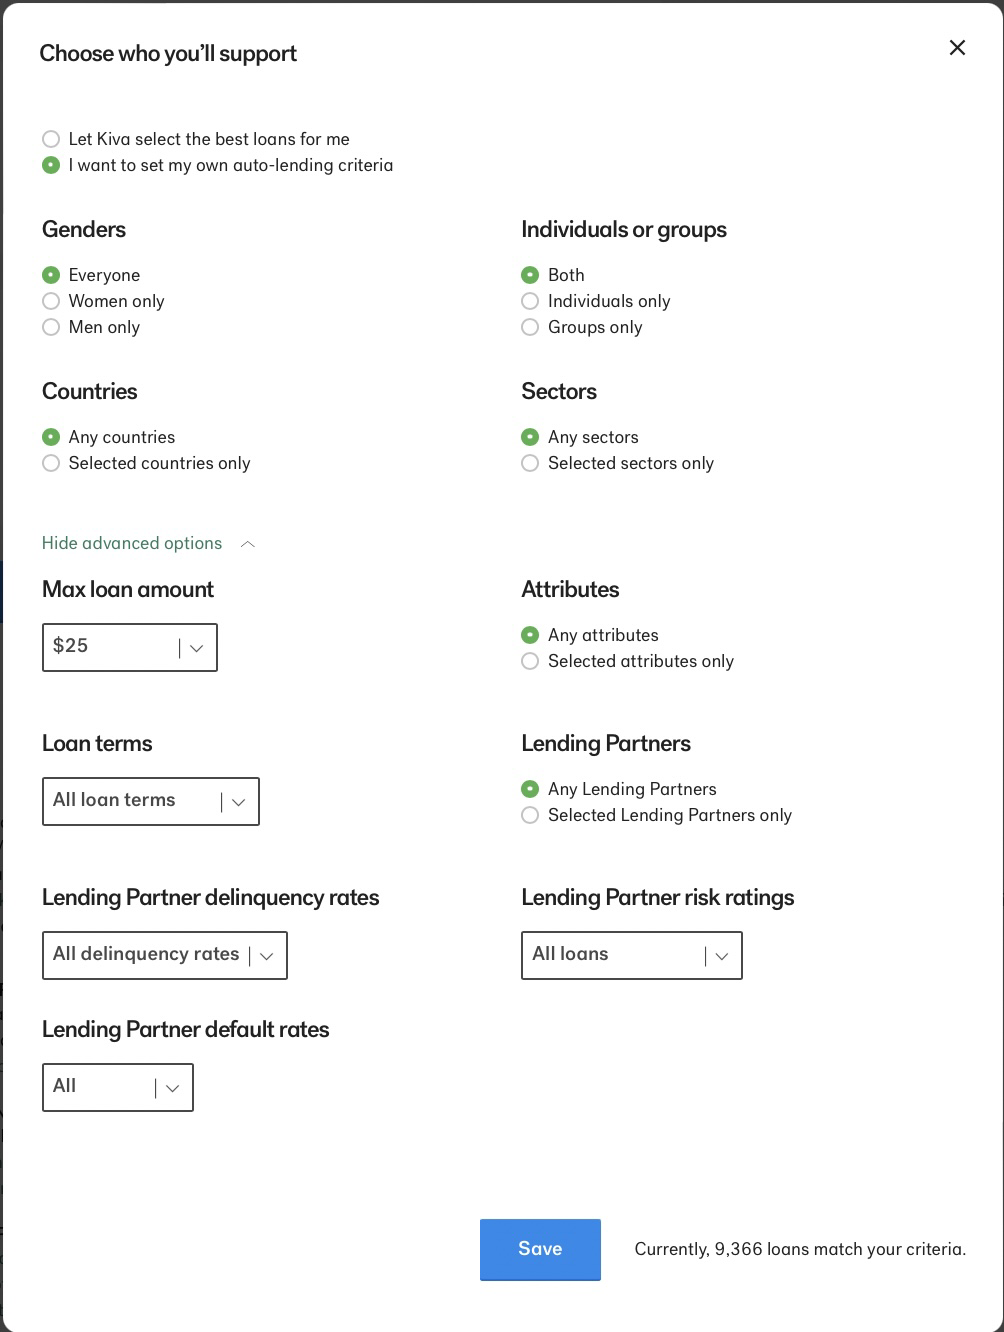
\includegraphics[width=0.8\textwidth]{images/auto-lend-setup.png}
	\caption{Auto-Lending setup interface \cite{kiva-autolend2}}
	\label{fig:auto-lend-setup}
\end{figure}

Users can "Let Kiva select the best loans for me" or "I want to set my own auto-lending criteria".
We do not have any information about how the platform select the best loans for users.
So we will focus on the second option.
We can see that the criterias are very similar to the criterias that users can use to search for projects.

\subsection{Kiva Data Access}

In order to access the data provided by Kiva, we utilize the GraphQL API.
Kiva has made their data available through this API, allowing developers to query and retrieve specific information from the platform.
This is perhap unique to Kiva, as most other crowdfunding platforms do not provide such access to their data.
It is also note that Kiva also provides a public dataset through their so called "Data Snapshot".
However, this function is appearantly not working at the time of writing.
There also another way to get the data from kiva website, which is through Web Crawling.
By analysis the website interface and the network traffic, we can get the data that the website use to display the information.
This approach is although popular, but it is not very reliable because the website can change its interface at any time.
In this thesis, we will focus on the GraphQL API.

GraphQL is a query language for APIs that provides a flexible and efficient way to request and manipulate data.
It allows us to specify the exact data we need and retrieve it in a single request, reducing the amount of network traffic and improving performance.
By leveraging the GraphQL API, we can easily access various data points such as borrower information, loan details, lender statistics, and more.
This enables us to perform in-depth analysis and gain valuable insights from the Kiva dataset.
The availability of Kiva's data through GraphQL provides us with a powerful tool to explore and analyze the platform's data in a convenient and efficient manner.

There are two noteworthy points about the GraphQL API.
The first is through the \textit{introspection} \cite{graphql-introspection} feature of GraphQL,
we could have the information of what queries that the platform supports,
as long as with the data schema.
The second is that we can ultilize the GraphQL API to get the data in a batched manner.
Usually the platform will limit the number of requests that a user can make to the API.
But if we use some Web Crawling techniques, we can manage to get all the data that avaliable in the API.

Kiva GraphQL API can be found publicly at \url{https://api.kivaws.org/graphql}.
One can connect to the URI with any compatible GraphQL client.
On top of that, kiva also use \textit{GraphQLi}, a web interface for easy try the GraphQL queries.
\ref{fig:grapqli} is the screenshot of the web interface.
We use the interface to introspection the data schema and to try out some queries before actually implementing them in the code.

\begin{figure}[H]
	\centering
	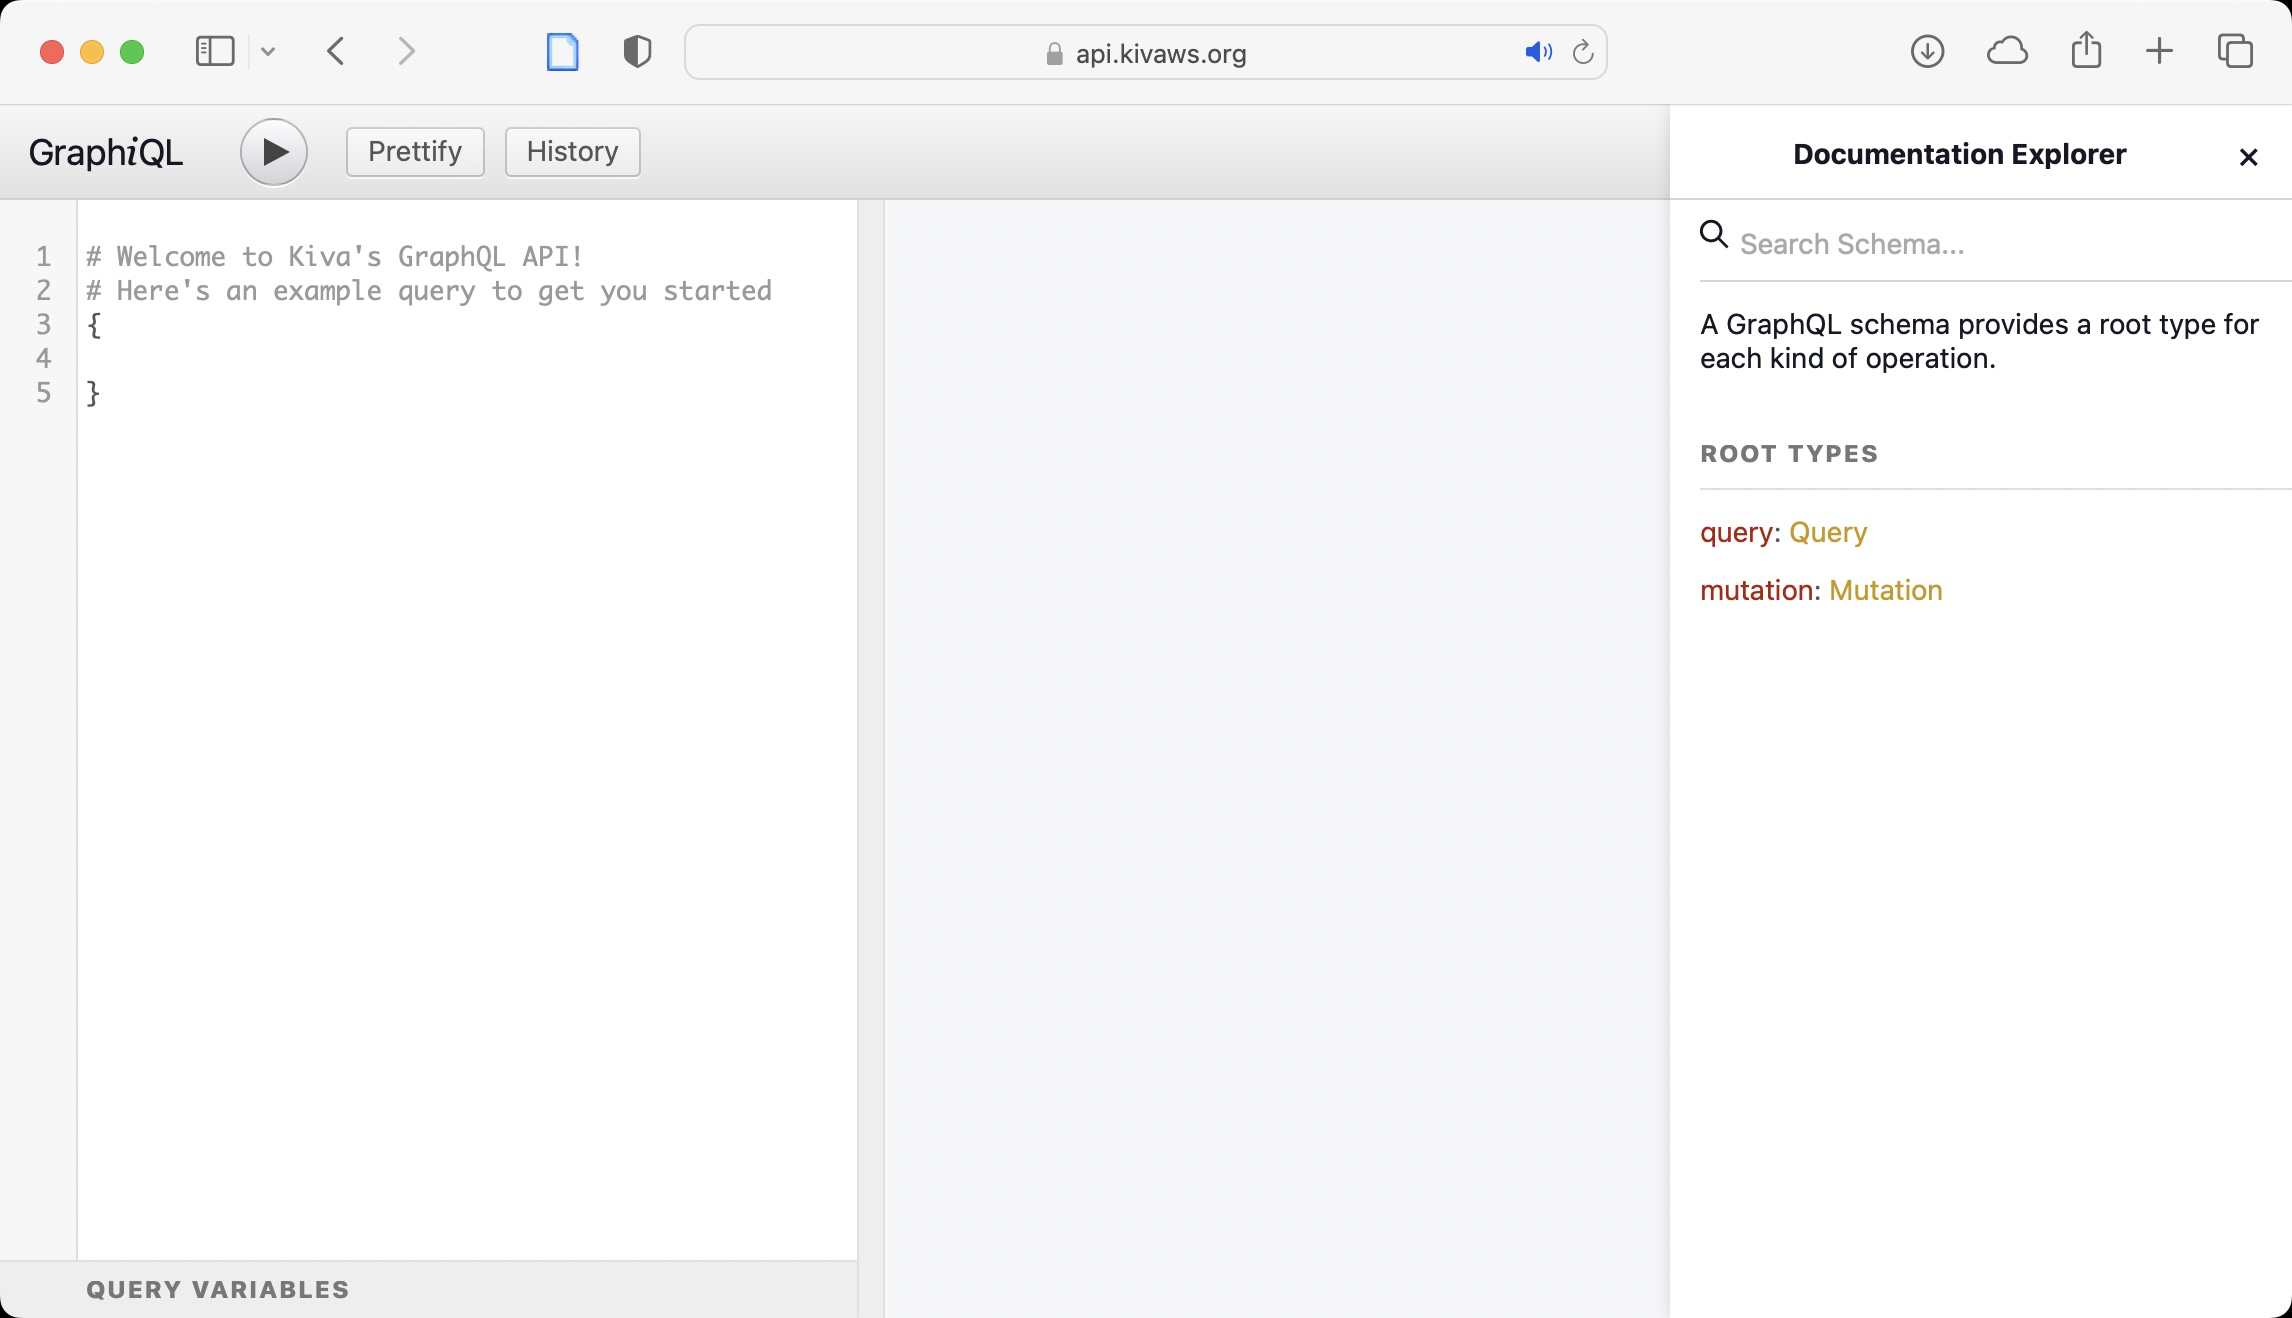
\includegraphics[width=0.8\textwidth]{images/grapqli.png}
	\caption{GraphQLi interface of Kiva GraphQL API}
	\label{fig:grapqli}
\end{figure}

For example, we could try the query for getting basic stats of kiva like following Figure.

\begin{figure}[H]
	\centering
	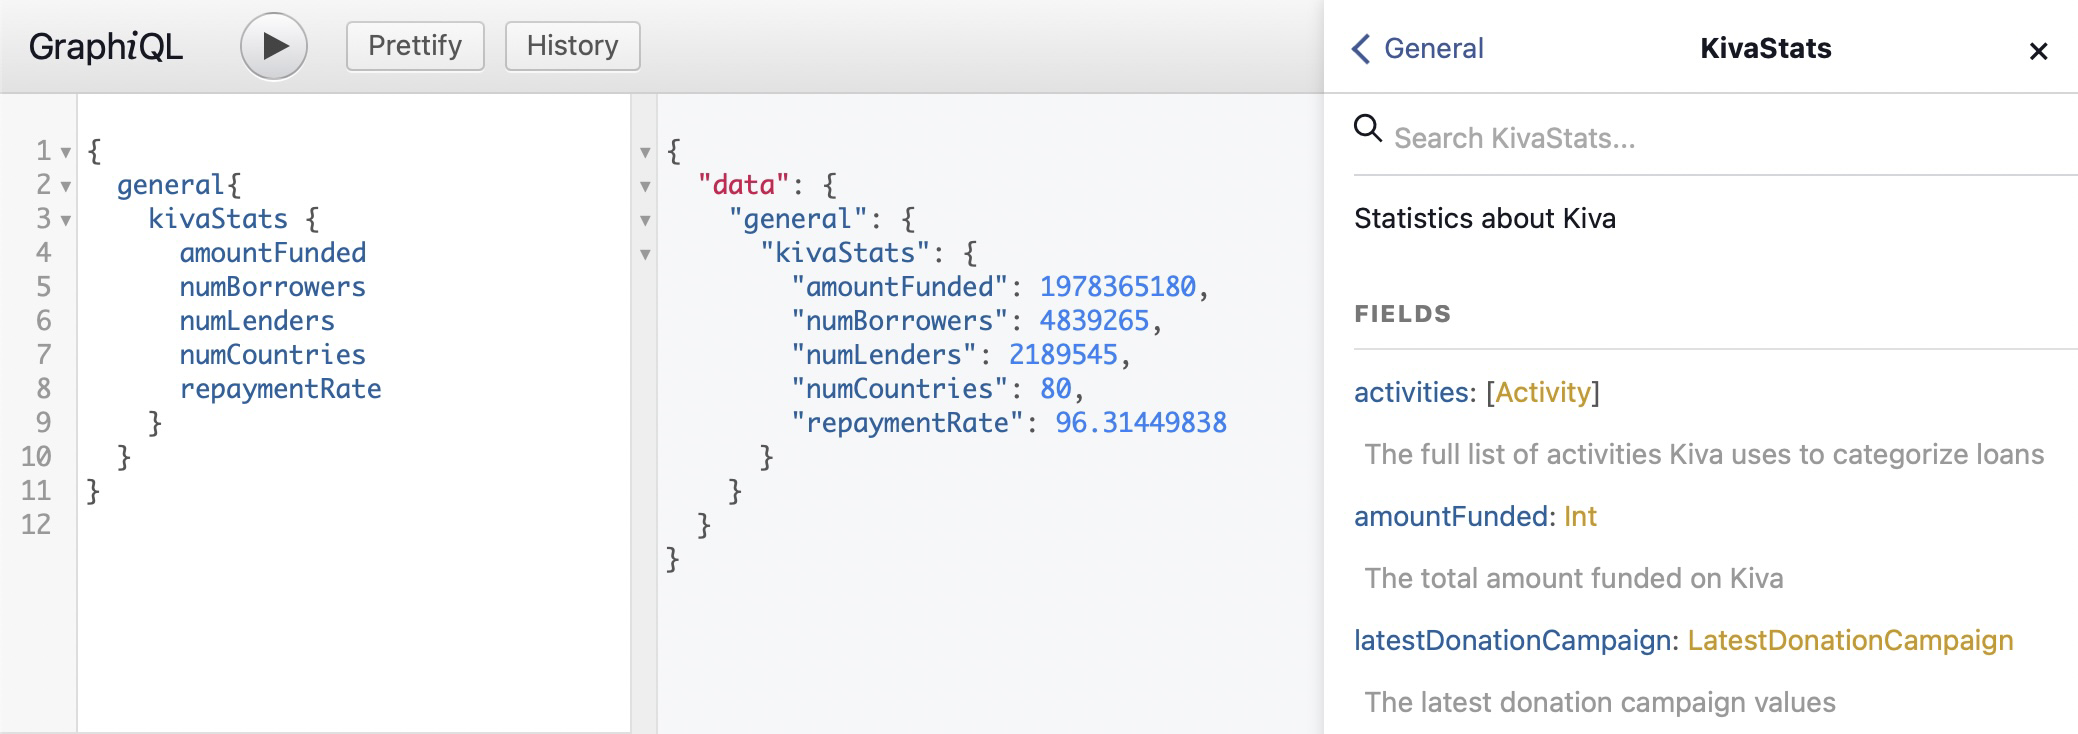
\includegraphics[width=0.8\textwidth]{images/graphqli-example.png}
	\caption{Example using GraphQLi interface of Kiva GraphQL API \cite{graphqli-example}}
	\label{fig:graphqli-example}
\end{figure}




Before begining to query the data, we have to understand the data schema to know what data that we can get.




\section{Basic data statistics}

\begin{itemize}
	\item Worldwide statistics
	      \begin{itemize}
		      \item How many projects
		      \item how many lenders
		      \item projects vs country distribution
		      \item successful rate
		      \item \textbf{How long that users stay on the platform}
	      \end{itemize}
	\item Vietnam statistics
	      \begin{itemize}
		      \item How many projects
		      \item \dots
	      \end{itemize}
\end{itemize}